\chapter{Detalles de implementación} \label{chap:implementacion}

\section{Consideraciones generales} \label{sect:implementacion-consideraciones}

\subsection{Lenguaje de programación} \label{sect:implementacion-lenguaje}

El lenguaje de programación utilizado para la implementación de las seis metaheurísticas fue C++, compilado usando g++ en su versión 4.4.3.

\subsection{Estructura de datos para la representación de una solución} \label{sect:implementacion-estructura}

Para representar una solución de VRPSPD se utilizó la estructura de datos propuesta por \cite{tesisdanielernesto}. Esta estructura ocupa $O(K + N)$ de espacios de memoria y está conformada por los siguientes elementos:

\begin{itemize}
\item \textbf{Arreglo de inicio: } arreglo de tamaño $K$ que contiene el primer cliente visitado por cada uno de los vehículos. Como los vehículos siempre parten del depósito en VRPSPD se asume que antes del primer cliente visitado se partió del depósito. Si es cero ($0$) es porque no existen más vehículos.
\item \textbf{Arreglo del próximo cliente: } arreglo de tamaño $N$ que contiene los clientes visitados por cada uno de los vehículos, exceptuando los almacenados en el arreglo anterior.
\end{itemize}

%\item \textbf{Arreglo inverso de inicio: } arreglo de tamaño K que contiene el último cliente visitado por cada uno de los vehículos (antes del depósito).
%\item \textbf{Arreglo inverso del próximo cliente: } arreglo de tamaño N que contiene los clientes visitados por cada uno de los vehículos con orden inverso, exceptuando los almacenados en el arreglo anterior.
%\item \textbf{Arreglo de capacidad de entrega inicial: } arreglo de tamaño K que contiene la capacidad ocupada en bienes de entrega en un vehículo antes de partir del depósito.
%\item \textbf{Arreglo de capacidad de recepción final: } arreglo de tamaño K que contiene la capacidad ocupada en bienes de recepción en un vehículo luego de llegar al depósito.
%\item \textbf{Arreglo de capacidad de entrega: } arreglo de tamaño N que contiene la capacidad ocupada en bienes de entrega en un vehículo antes de atender a un cliente determinado.
%\item \textbf{Arreglo de capacidad de recepción: } arreglo de tamaño N que contiene la capacidad ocupada en bienes de recepción en un vehículo antes de atender a un cliente determinado.
%\end{itemize}

La \textbf{Figura~\ref{VRP_representation}} muestra una solución de VRPSPD y su representación utilizando la estructura de datos men\-cio\-na\-da. Para construir la ruta recorrida por un vehículo se debe comenzar por obtener el primer cliente visitado de ese vehículo luego del depósito utilizando el \emph{Arreglo de inicio} e iterativamente construir el resto de la ruta con la información en los campos correspondientes al \emph{Arreglo del próximo cliente}, hasta encontrar el depósito (usualmente denotado como cliente 0). 


\begin{figure}[h]
	\begin{center}
		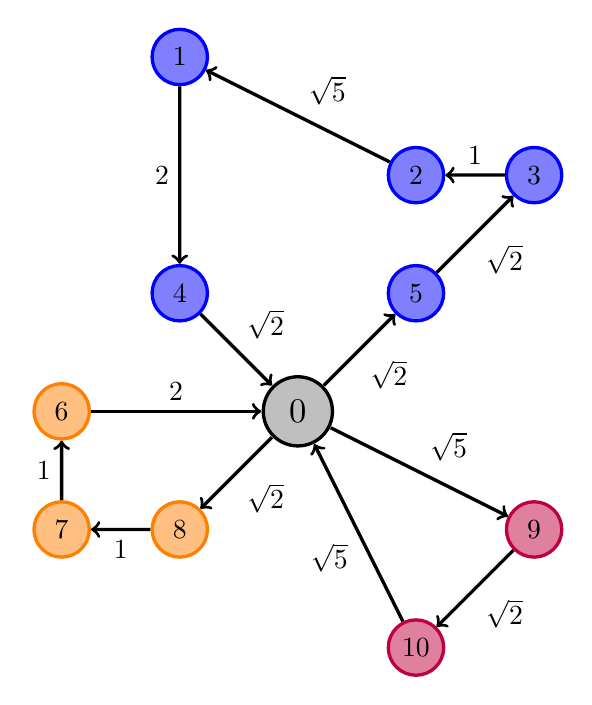
\begin{tikzpicture}[scale=1.5, auto, very thick]
			\tikzstyle{vertex}   = [circle, minimum size=20pt, inner sep=0pt, draw=black, fill=black!25, scale=1.25]
			\tikzstyle{vertexA}  = [circle, minimum size=20pt, inner sep=0pt, draw=purple, fill=purple!50]
			\tikzstyle{vertexB}  = [circle, minimum size=20pt, inner sep=0pt, draw=blue, fill=blue!50]
			\tikzstyle{vertexC}  = [circle, minimum size=20pt, inner sep=0pt, draw=orange, fill=orange!50]
			\tikzstyle{vertexA2} = [circle, minimum size=20pt, inner sep=0pt, draw=purple, fill=purple!50]
			\tikzstyle{vertexB2} = [circle, minimum size=20pt, inner sep=0pt, draw=blue, fill=blue!50]
			\tikzstyle{vertexC2} = [circle, minimum size=20pt, inner sep=0pt, draw=orange, fill=orange!50]
			
%			\draw[step=1cm, gray!50] (-2.4,-2.4) grid (2.4,3.4);

			\node[vertex] (dep) at (0, 0) {$0$};
%TODO		\node[] at (0, -5) {$a$};
			\foreach \text/\x/\y/\styl in {9/2/-1/A, 5/1/1/B, 3/2/2/B, 2/1/2/B, 1/-1/3/B, 7/-2/-1/C, 8/-1/-1/C, 10/1/-2/A2, 4/-1/1/B2, 6/-2/0/C2}
				\node[vertex\styl] (\text) at (\x, \y) {$\text$};
			
			\foreach \from/\to/\cost in {dep/9/\sqrt{5}, 9/10/\sqrt{2}, 10/dep/\sqrt{5}, 4/dep/\sqrt{2}, dep/8/\sqrt{2}, 8/7/1, 7/6/1, 6/dep/2}
				\path[<-] (\to) edge node [swap] {$\cost$} (\from);

			\foreach \from/\to/\cost in {dep/5/\sqrt{2}, 5/3/\sqrt{2}, 3/2/1, 2/1/\sqrt{5}, 1/4/2}
				\path[<-] (\to) edge node {$\cost$} (\from);
		\end{tikzpicture}
		\hspace{.25in}
		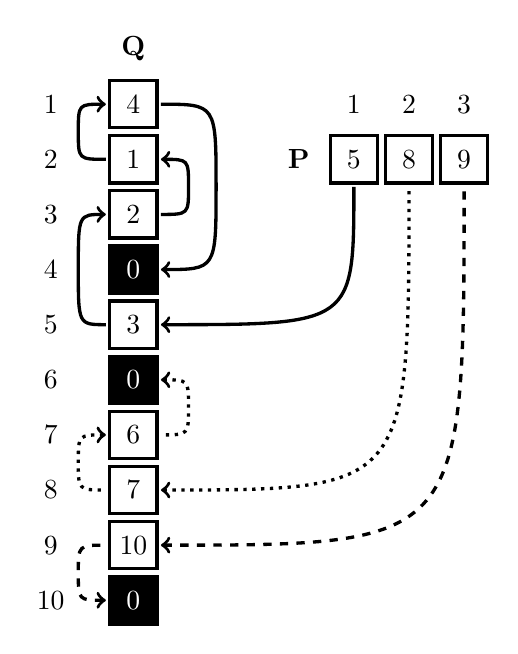
\begin{tikzpicture}[scale=0.7, auto, very thick]
			\tikzstyle{square} = [rectangle, draw, minimum height=20pt, minimum width=20pt, text centered]

			\node (veh) at (5, -2) {\textbf{P}};
			\node (veh) at (2,  0) {\textbf{Q}};
			
			\foreach \index/\text in {1/5, 2/8, 3/9} {
				\draw (5 + \index, -2) node[fill=white, minimum size=0.6cm, draw] {};
				\node (I-\index) at (5 + \index, -1) {$\index$};
				\node[text=black] (Q-\index) at (5 + \index, -2) {$\text$};
			}

			\foreach \index/\text in {1/4, 2/1, 3/2, 5/3, 7/6, 8/7, 9/10} {
				\draw (2, -\index) node[minimum size=0.6cm, draw] {};
				\node (I-\index) at (.5, -\index) {$\index$};
				\node (Q-\index) at (2, -\index) {$\text$};
			}

			\foreach \index/\text in {4/0, 6/0, 10/0} {
				\draw (2, -\index) node[fill=black, minimum size=0.6cm, draw] {};
				\node (I-\index) at (.5, -\index) {$\index$};
				\node[text=white] (Q-\index) at (2, -\index) {$\text$};
			}

			\draw[<-] (2.5, -5) .. controls (6, -5) .. (6, -2.5);
			\draw[<-] (1.5, -3) .. controls (1, -3) .. (1, -4) .. controls (1, -5) .. (1.5, -5);
			\draw[<-] (2.5, -2) .. controls (3, -2) .. (3, -2.5) .. controls (3, -3) .. (2.5, -3);
			\draw[<-] (1.5, -1) .. controls (1, -1) .. (1, -1.5) .. controls (1, -2) .. (1.5, -2);
			\draw[<-] (2.5, -4) .. controls (3.5, -4) .. (3.5, -2.5) .. controls (3.5, -1) .. (2.5, -1);

			\draw[<-, dashed] (2.5, -9) .. controls (8, -9) .. (8, -2.5);
			\draw[<-, dashed] (1.5, -10) .. controls (1, -10) .. (1, -9.5) .. controls (1, -9) .. (1.5, -9);
			
			\draw[<-, dotted] (2.5, -8) .. controls (7, -8) .. (7, -2.5);
			\draw[<-, dotted] (1.5, -7) .. controls (1, -7) .. (1, -7.5) .. controls (1, -8) .. (1.5, -8);
			\draw[<-, dotted] (2.5, -6) .. controls (3, -6) .. (3, -6.5) .. controls (3, -7) .. (2.5, -7);
		\end{tikzpicture}
	\end{center}
	\caption[Representación de una Solución de VRPSPD]{\textsl{Representación de una Solución de VRPSPD}. $P$ es el arreglo de \textsl{Inicio} y $Q$ es el arreglo del \textsl{Próximo Cliente}. Los nodos circulares representan los clientes.}
	\label{VRP_representation}
\end{figure}


Un esquema general de como obtener la construcción de las rutas a partir de esta estructura de datos puede verse en  \textbf{Apéndice~\ref{chap:apendiceA}}, \textbf{Algoritmo~\ref{alg:ConstRutas}}.

%De la misma manera funcionan los arreglos de \emph{Arreglo inverso de inicio} y \emph{Arreglo inverso del próximo cliente} respectivamente.
%
%\emph{Arreglo de capacidad de entrega inicial} y \emph{Arreglo de capacidad de recepción final} contienen la información de la capacidad del vehículo correspondiente en bienes.
%
%\emph{Arreglo de capacidad de entrega} y \emph{Arreglo de capacidad de recepción} contienen la información de capacidad antes de visitar un cliente determinado.

\subsection{Algoritmos de generación de soluciones iniciales} \label{sect:implementacion-algoritmos-iniciales}

Las metaheurísticas de trayectoria y poblacionales necesitan de una solución inicial para poder realizar su trabajo. Los algoritmos utilizados para generar estas soluciones iniciales son los siguientes:

\begin{itemize}
\item \textbf{Algoritmo de inserción:} heurística de inserción basada en \cite{heuristicainsercion}. En un principio este algoritmo  crea un número predeterminado $r$ de rutas e inicializa una lista de candidatos LC. Luego inserta aleatoriamente un cliente t $\in $ LC en cada una de ellas. Más tarde realiza iterativamente la mejor inserción posible entre todos los clientes t $\in$ LC, tal que su función de evaluación tenga valor mínimo. Este último proceso se repite hasta $LC = \emptyset$. La función de evaluación se encuentra expresada en la siguiente ecuación:

\begin{equation}\label{eq:insercion}
f(t,r)= (c_{it}+c_{tj}-c_{ij}) - \gamma (c_{0t}+c_{t0})
\end{equation}

La primera parte de la ecuación está relacionada con el muy conocido criterio de inserción factible de menor costo, el cual  usa una estrategia ambiciosa que toma en cuenta el menor costo adicional de inserción del cliente $t$ entre el cliente $i$ y $j$ en la ruta $r$. Sólo se toman en cuenta inserciones factibles.   La segunda parte de la ecuación corresponde a un recargo utilizado para evitar que se inserten clientes que se encuentren ubicados remotamente del depósito. El costo de salir del depósito y regresar a él está condicionado por un factor $\gamma \in$ [0,1].

%El pseudocódigo general de este algoritmo de inserción se puede ver en el \textbf{Apéndice~\ref{chap:apendiceA}}, \textbf{Algoritmo~\ref{alg:AlgIns}}.

\item \textbf{Algoritmo de generación aleatoria:} inserta los clientes en una posición y ruta aleatorias. 

\item \textbf{Algoritmo de vecino más cercano:} se comienza creando una ruta vacía. Posteriormente se inserta el cliente que minimice el costo.  Luego se realiza la inserción factible del cliente adyacente que minimice el costo desde el cliente anterior a éste. Se repite el procedimiento anterior hasta que sea infactible agregar un nuevo cliente. En este escenario se reinicia completamente el procedimiento creando una nueva ruta vacía. Si no hay más clientes sin ser asignados a una ruta se finaliza el algoritmo.

\item \textbf{Algoritmo de construcción basado en ahorro de costos:} heurística de construcción basada en el ahorro de costos propuesto por \cite{savings}. Este algoritmo comienza creando una nueva ruta que contiene el depósito dos veces (origen y terminación de la ruta). Luego, el costo de insertar cada cliente (sin asignar) en cada posible posición factible es calculado. El costo de insertar el cliente $k$ entre los vertices $i$ y $j$ es obtenido por la ecuación:

\begin{equation}\label{eq:cost_savings}
costo_{ijk} = c_{ik} + c_{kj} - gc_{ij} + f|c_{ik} - c_{kj}|
\end{equation}

donde $g$ y $f$ son valores estocásticos tal que $g\in$ [0,3] y $f\in$ [0,1] según \cite{savings}, y dirigen la metodología de construcción a soluciones iniciales diversas.

Para cada cliente $i$, la inserción factible que minimice $costo$, denotada como $mcosto_i$ es identificada, y describe la inserción del cliente $i$ en la posición denominada $mp_i$ de la ruta $mr_i$. Sea $mc$ el cliente con el menor valor de $mcosto_i$, para cada cliente $j$ con $mr_j$=$mr_{mc}$ y $mp_j$=$mp_{mc}$, el costo de inserción $mcosto'_j$ es evaluado como $mcosto'_j=\lambda(c_{j0} + c_{0j}) - mcosto_j$, donde $\lambda$ está uniformemente distribuida y $\lambda\in$ [0,1] mientras que $c_{j0}$ y $c_{0j}$ denotan el costo de transición desde $j$ al depósito y desde el depósito a $j$ respectivamente. Sea $ins$ el cliente para el cual $mcosto'_j$ es mínimo, entonces el cliente $ins$ es asignado a la ruta $mr_{ins}$, en la posición $mp_{ins}$. Este procedimiento se repite iterativamente hasta que cada cliente sea asignado a alguna ruta. Si todas las inserciones son infactibles, se crea una ruta nueva disponible para insertar otros clientes.

\item \textbf{Algoritmo ambicioso de construcción aleatoria:} El procedimiento comienza abriendo la primera ruta (k = 1) y después crea una lista de candidatos con el valor de la función greedy de todos los clientes en el problema. El costo de cada camino es evaluado con una función que mide el incremento de la distancia recorrida al agregar un nuevo cliente. Nuevas rutas son creadas cuando la ruta llega al límite de la capacidad permitida.  Sea i el índice del último cliente visitado por el vehículo k en la solución parcial actual. Además, sea j el cliente candidato para ser agregado a la ruta, inmediatamente luego del cliente i. Luego el valor de la función greedy para el cliente asociado j se da por la siguiente fórmula:
  	
\begin{equation}\label{eq:cost_savings}
c_{ij} = d_{ij} + d_{j0} 
\end{equation}
  	
  	
	Donde $d_{ij}$ es la distancia entre el cliente i y el cliente j y $d_{j0}$ denota el la distancia entre el cliente j y el depósito. El procedimiento solo considera como candidatos aquellos clientes que no hayan sido visitados hasta el momento y que no incumplan con la restricción de capacidad. Sea i el último cliente visitado en la ruta actual y j un cliente candidato, se obtiene de la lista de candidatos el $c_{i,j}$, $c_{min}$ y el $c_{max}$ , para luego tomar aleatoriamente alguno de ellos que cumpla con la siguiente ecuación: 
	
\begin{equation}\label{eq:cost_savings}
c_{i,j} \leqslant c_{min} + \alpha(c_{min} + c_{max}) 
\end{equation}

	Si ningúno de los clientes restantes es parte de la lista de candidatos, entonces se comienza una ruta nueva incrementando en uno el valor de k. 

\end{itemize}


\section{Heurísticas y metaheurísticas} \label{sect:implementacion-heuristicas}

En esta sección se presentan las heurísticas y metaheurísticas que fueron utilizadas en las metaheurísticas implementadas como métodos de mejoramiento e hibridación.

\subsection{Búsqueda local} \label{sect:implementacion-busquedalocal}

Se implementó búsqueda local con estrategia \emph{mejor-mejor}, es decir, se busca la mejor solución posible que pertenezca a la vecindad.

\subsection*{Operadores de vecindad utilizados}

La mayor parte de los operadores implementados provienen  de \cite{operadoresLS}, excepto reverse e interchange que fueron utilizados en \cite{SalhiNagyLS} y \cite{gts} respectivamente. Es importante destacar que todos los operadores de vecindad solo realizan cambios factibles dentro de una solución. Los operadores se aplican de dos formas: \emph{intra-ruta} e \emph{inter-ruta}. Un operador \emph{intra-ruta} realiza cambios de clientes dentro de una ruta. Mientras que un operador \emph{inter-ruta} realiza cambios de clientes entre rutas distintas. 

A continuación se presenta una lista de los operadores generadores de vecindades implementados, de los cuales los inter-ruta se representan en la \textbf{Figura~\ref{Oper-inter}} y los intra-ruta en la \textbf{Figura~\ref{Oper-intra}}:

\subsubsection*{Operadores intra-ruta:}
\begin{itemize}
\item \textbf{Swap:} intercambia la posición del cliente $n_i$ con la posición de otro cliente $n_j$.
\item \textbf{Or-opt:} toma el cliente localizado en la posición $p_i$ y lo inserta en la posición $p_j$. Este operador fue im\-ple\-men\-ta\-do para realizar la relocalización de uno, dos o tres clientes adyacentes.
\item \textbf{2-opt:} elimina dos arcos y crea dos arcos distintos entre los clientes que quedan sin arcos invirtiendo el orden del camino entre los arcos generados. 
\item \textbf{Reverse:} invierte la dirección de la ruta en caso de que este cambio reduzca la máxima carga de la ruta correspondiente.
\end{itemize}

\subsubsection*{Operadores inter-ruta:}
\begin{itemize}
\item \textbf{Swap:} intercambia la posición del cliente $n_i$ en la ruta $r_k$ con la posición de otro cliente $n_j$ en la ruta $r_l$.
\item \textbf{Shift:} toma el cliente localizado en la posición $p_i$ de la ruta $r_k$ y lo inserta en la posición $p_j$ de la ruta $r_l$. Este operador fue implementado para realizar la relocalización de uno o dos clientes contiguos.
\item \textbf{Crossover:} divide las rutas $r_i$ y $r_j$ en dos partes: inicial y final. Luego conecta la parte inicial de la ruta $r_i$ con la parte final de la ruta $r_j$, así como la parte inicial de la ruta $r_j$ es enlazada con la parte inicial de la ruta $r_i$.
\item \textbf{Interchange:} divide las rutas $r_i$ y $r_j$ en dos partes: inicial y final. Luego conecta la parte inicial de la ruta $r_i$ con la parte inicial de la ruta $r_j$, así como la parte final de la ruta $r_j$ es enlazada con la parte final de la ruta $r_i$ invirtiendo el camino generado.
\end{itemize}

\begin{figure}[ht]
	\centering
	\subfloat[Shift]{\label{oper:shi}
		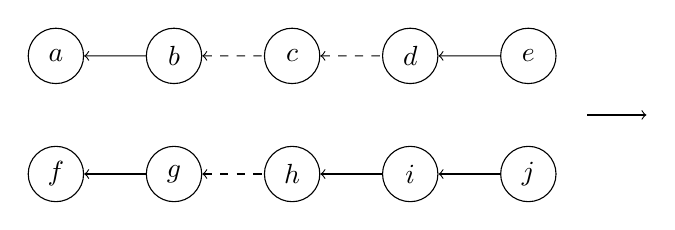
\begin{tikzpicture}[scale=0.75]
			\tikzstyle{vertex}  = [circle, minimum size=20pt, inner sep=0pt, draw=black, fill=white]
			
			\foreach \text/\x/\y in {a/0/2, b/2/2, c/4/2, d/6/2, e/8/2, f/0/0, g/2/0, h/4/0, i/6/0, j/8/0}
				\node[vertex] (\text) at (\x, \y) {$\text$};

			\foreach \from/\to in {a/b, d/e, f/g, h/i, i/j}
				\path[<-] (\from) edge node {} (\to);

			\foreach \from/\to in {b/c, c/d, g/h}
				\path[<-, dashed] (\from) edge node {} (\to);
			
			\draw[<-] (10, 1) -- (9, 1);
		\end{tikzpicture}
		
		\hspace{.2cm}

		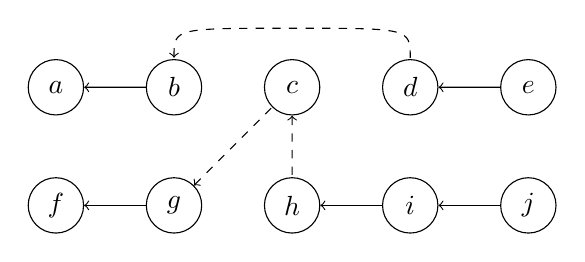
\begin{tikzpicture}[scale=0.75]
			\tikzstyle{vertex}  = [circle, minimum size=20pt, inner sep=0pt, draw=black, fill=white]
			
			\foreach \text/\x/\y in {a/0/2, b/2/2, c/4/2, d/6/2, e/8/2, f/0/0, g/2/0, h/4/0, i/6/0, j/8/0}
				\node[vertex] (\text) at (\x, \y) {$\text$};

			\foreach \from/\to in {a/b, d/e, f/g, h/i, i/j}
				\path[<-] (\from) edge node {} (\to);

			\foreach \from/\to in {g/c, c/h}
				\path[<-, dashed] (\from) edge node {} (\to);

			\draw[<-, dashed] (2, 2.5) .. controls (2, 3) .. (4, 3) .. controls (6, 3) .. (6, 2.5);
		\end{tikzpicture}

	}	
	
	\subfloat[Swap]{\label{oper:swp}
		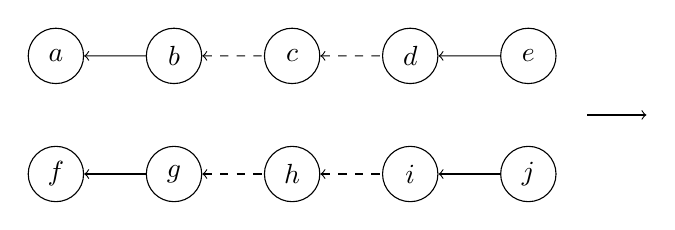
\begin{tikzpicture}[scale=0.75]
			\tikzstyle{vertex}  = [circle, minimum size=20pt, inner sep=0pt, draw=black, fill=white]
			
			\foreach \text/\x/\y in {a/0/2, b/2/2, c/4/2, d/6/2, e/8/2, f/0/0, g/2/0, h/4/0, i/6/0, j/8/0}
				\node[vertex] (\text) at (\x, \y) {$\text$};

			\foreach \from/\to in {a/b, d/e, f/g, i/j}
				\path[<-] (\from) edge node {} (\to);

			\foreach \from/\to in {b/c, c/d, g/h, h/i}
				\path[<-, dashed] (\from) edge node {} (\to);

			\draw[<-] (10, 1) -- (9, 1);
		\end{tikzpicture}

		\hspace{.2cm}

		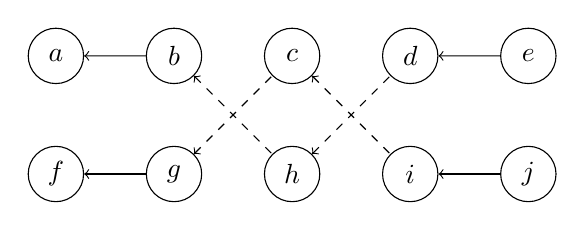
\begin{tikzpicture}[scale=0.75]
			\tikzstyle{vertex}  = [circle, minimum size=20pt, inner sep=0pt, draw=black, fill=white]
			
			\foreach \text/\x/\y in {a/0/2, b/2/2, c/4/2, d/6/2, e/8/2, f/0/0, g/2/0, h/4/0, i/6/0, j/8/0}
				\node[vertex] (\text) at (\x, \y) {$\text$};

			\foreach \from/\to in {a/b, d/e, f/g, i/j}
				\path[<-] (\from) edge node {} (\to);

			\foreach \from/\to in {g/c, c/i, b/h, h/d}
				\path[<-, dashed] (\from) edge node {} (\to);
		\end{tikzpicture}
	}
	
	\subfloat[Crossover]{\label{oper:cross}
		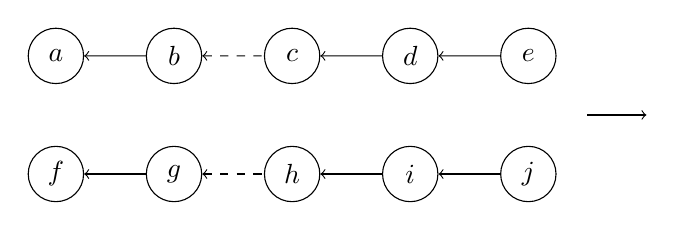
\begin{tikzpicture}[scale=0.75]
			\tikzstyle{vertex}  = [circle, minimum size=20pt, inner sep=0pt, draw=black, fill=white]
			
			\foreach \text/\x/\y in {a/0/2, b/2/2, c/4/2, d/6/2, e/8/2, f/0/0, g/2/0, h/4/0, i/6/0, j/8/0}
				\node[vertex] (\text) at (\x, \y) {$\text$};

			\foreach \from/\to in {a/b, c/d, d/e, f/g, h/i, i/j}
				\path[<-] (\from) edge node {} (\to);

			\foreach \from/\to in {b/c, g/h}
				\path[<-, dashed] (\from) edge node {} (\to);

			\draw[<-] (10, 1) -- (9, 1);
		\end{tikzpicture}

		\hspace{.2cm}

		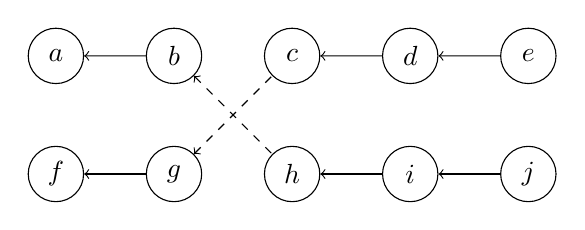
\begin{tikzpicture}[scale=0.75]
			\tikzstyle{vertex}  = [circle, minimum size=20pt, inner sep=0pt, draw=black, fill=white]
			
			\foreach \text/\x/\y in {a/0/2, b/2/2, c/4/2, d/6/2, e/8/2, f/0/0, g/2/0, h/4/0, i/6/0, j/8/0}
				\node[vertex] (\text) at (\x, \y) {$\text$};

			\foreach \from/\to in {a/b, c/d, d/e, f/g, h/i, i/j}
				\path[<-] (\from) edge node {} (\to);

			\foreach \from/\to in {g/c, b/h}
				\path[<-, dashed] (\from) edge node {} (\to);
		\end{tikzpicture}
	}		
			
	\subfloat[Interchange]{\label{oper:inter}
		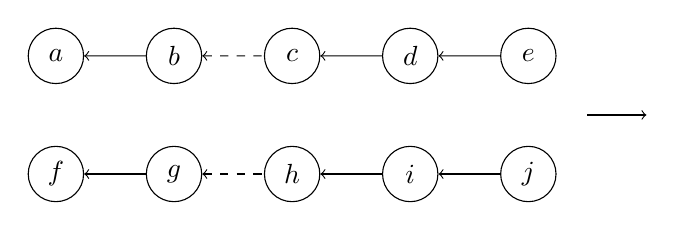
\begin{tikzpicture}[scale=0.75]
			\tikzstyle{vertex}  = [circle, minimum size=20pt, inner sep=0pt, draw=black, fill=white]
			
			\foreach \text/\x/\y in {a/0/2, b/2/2, c/4/2, d/6/2, e/8/2, f/0/0, g/2/0, h/4/0, i/6/0, j/8/0}
				\node[vertex] (\text) at (\x, \y) {$\text$};

			\foreach \from/\to in {a/b, c/d, d/e, f/g, h/i, i/j}
				\path[<-] (\from) edge node {} (\to);

			\foreach \from/\to in {b/c, g/h}
				\path[<-, dashed] (\from) edge node {} (\to);

			\draw[<-] (10, 1) -- (9, 1);
		\end{tikzpicture}

		\hspace{.2cm}

		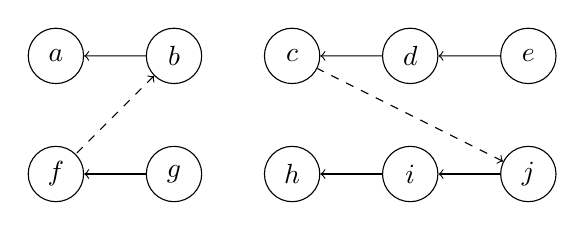
\begin{tikzpicture}[scale=0.75]
			\tikzstyle{vertex}  = [circle, minimum size=20pt, inner sep=0pt, draw=black, fill=white]
			
			\foreach \text/\x/\y in {a/0/2, b/2/2, c/4/2, d/6/2, e/8/2, f/0/0, g/2/0, h/4/0, i/6/0, j/8/0}
				\node[vertex] (\text) at (\x, \y) {$\text$};

			\foreach \from/\to in {a/b, c/d, d/e, f/g, h/i, i/j}
				\path[<-] (\from) edge node {} (\to);

			\foreach \from/\to in {j/c, b/f}
				\path[<-, dashed] (\from) edge node {} (\to);
		\end{tikzpicture}
	}	
			
	\caption{Operadores inter-ruta de generación de vecindades.}
	\label{Oper-inter}
\end{figure}

\begin{figure}[ht]
	\centering
	\subfloat[2-opt]{\label{oper:2-opt}
		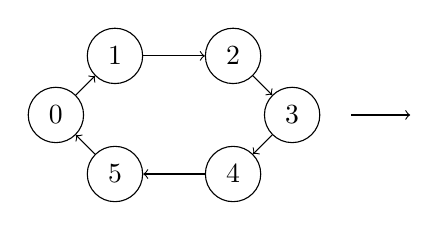
\begin{tikzpicture}[scale=0.75]
			\tikzstyle{vertex}  = [circle, minimum size=20pt, inner sep=0pt, draw=black, fill=white]
		
			
%			\draw[step=1cm, gray!50] (-2.4,-2.4) grid (2.4,3.4);

			\node[vertex] (dep) at (0, 0) {$0$};
			
			\foreach \text/\x/\y in {1/1/1, 2/3/1, 3/4/0, 4/3/-1, 5/1/-1}
				\node[vertex] (\text) at (\x, \y) {$\text$};
			
			\foreach \from/\to in {dep/1, 1/2, 2/3, 3/4, 4/5, 5/dep}
				\path[<-] (\to) edge node [swap] {} (\from);
		
		\draw[<-] (6, 0) -- (5, 0);
		\end{tikzpicture}
		
		\hspace{.2cm}				
		
		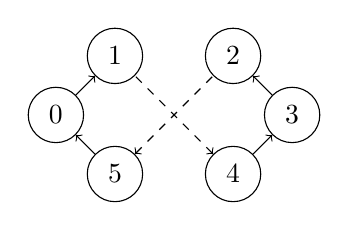
\begin{tikzpicture}[scale=0.75]
			\tikzstyle{vertex}  = [circle, minimum size=20pt, inner sep=0pt, draw=black, fill=white]
			
%			\draw[step=1cm, gray!50] (-2.4,-2.4) grid (2.4,3.4);

			\node[vertex] (dep) at (0, 0) {$0$};
			
			\foreach \text/\x/\y in {1/1/1, 2/3/1, 3/4/0, 4/3/-1, 5/1/-1}
				\node[vertex] (\text) at (\x, \y) {$\text$};
			
			\foreach \from/\to in {dep/1, 4/3, 3/2, 5/dep}
				\path[<-] (\to) edge node [swap] {} (\from);
			
			\foreach \from/\to in {4/1, 5/2}
				\path[<-, dashed] (\from) edge node {} (\to);	

		\end{tikzpicture}		
		
	}

	\subfloat[Swap]{\label{oper:intra-swap}
		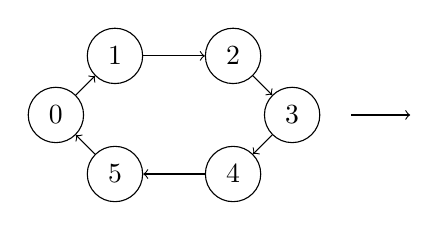
\begin{tikzpicture}[scale=0.75]
			\tikzstyle{vertex}  = [circle, minimum size=20pt, inner sep=0pt, draw=black, fill=white]
		
			
%			\draw[step=1cm, gray!50] (-2.4,-2.4) grid (2.4,3.4);

			\node[vertex] (dep) at (0, 0) {$0$};
			
			\foreach \text/\x/\y in {1/1/1, 2/3/1, 3/4/0, 4/3/-1, 5/1/-1}
				\node[vertex] (\text) at (\x, \y) {$\text$};
			
			\foreach \from/\to in {dep/1, 1/2, 2/3, 3/4, 4/5, 5/dep}
				\path[<-] (\to) edge node [swap] {} (\from);
		
		\draw[<-] (6, 0) -- (5, 0);
		\end{tikzpicture}
		
		\hspace{.2cm}				
		
		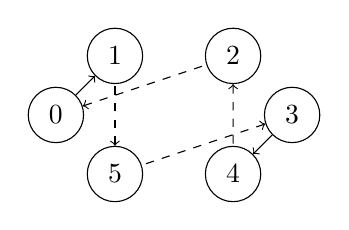
\begin{tikzpicture}[scale=0.75]
			\tikzstyle{vertex}  = [circle, minimum size=20pt, inner sep=0pt, draw=black, fill=white]
			
%			\draw[step=1cm, gray!50] (-2.4,-2.4) grid (2.4,3.4);

			\node[vertex] (dep) at (0, 0) {$0$};
			
			\foreach \text/\x/\y in {1/1/1, 2/3/1, 3/4/0, 4/3/-1, 5/1/-1}
				\node[vertex] (\text) at (\x, \y) {$\text$};
			
			\foreach \from/\to in {dep/1, 3/4}
				\path[<-] (\to) edge node [swap] {} (\from);
			
			\foreach \from/\to in {5/1, 3/5, dep/2, 2/4}
				\path[<-, dashed] (\from) edge node {} (\to);	

		\end{tikzpicture}		
		
	}

	\subfloat[Or-opt]{\label{oper:intra-or}
		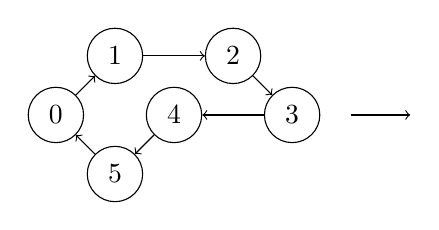
\begin{tikzpicture}[scale=0.75]
			\tikzstyle{vertex}  = [circle, minimum size=20pt, inner sep=0pt, draw=black, fill=white]
		
			
%			\draw[step=1cm, gray!50] (-2.4,-2.4) grid (2.4,3.4);

			\node[vertex] (dep) at (0, 0) {$0$};
			
			\foreach \text/\x/\y in {1/1/1, 2/3/1, 3/4/0, 4/2/0, 5/1/-1}
				\node[vertex] (\text) at (\x, \y) {$\text$};
			
			\foreach \from/\to in {dep/1, 1/2, 2/3, 3/4, 4/5, 5/dep}
				\path[<-] (\to) edge node [swap] {} (\from);
		
		\draw[<-] (6, 0) -- (5, 0);
		\end{tikzpicture}
		
		\hspace{.2cm}				
		
		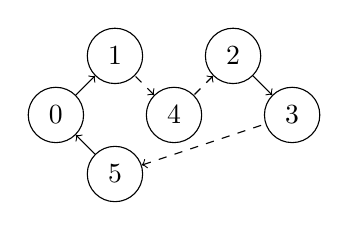
\begin{tikzpicture}[scale=0.75]
			\tikzstyle{vertex}  = [circle, minimum size=20pt, inner sep=0pt, draw=black, fill=white]
			
%			\draw[step=1cm, gray!50] (-2.4,-2.4) grid (2.4,3.4);

			\node[vertex] (dep) at (0, 0) {$0$};
			
			\foreach \text/\x/\y in {1/1/1, 2/3/1, 3/4/0, 4/2/0, 5/1/-1}
				\node[vertex] (\text) at (\x, \y) {$\text$};
			
			\foreach \from/\to in {dep/1, 2/3, 5/dep}
				\path[<-] (\to) edge node [swap] {} (\from);
			
			\foreach \from/\to in {5/3, 2/4, 4/1}
				\path[<-, dashed] (\from) edge node {} (\to);	

		\end{tikzpicture}		
		
	}
	
		\subfloat[Reverse]{\label{oper:reverse}
		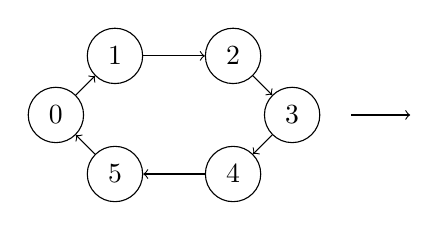
\begin{tikzpicture}[scale=0.75]
			\tikzstyle{vertex}  = [circle, minimum size=20pt, inner sep=0pt, draw=black, fill=white]
		
			
%			\draw[step=1cm, gray!50] (-2.4,-2.4) grid (2.4,3.4);

			\node[vertex] (dep) at (0, 0) {$0$};
			
			\foreach \text/\x/\y in {1/1/1, 2/3/1, 3/4/0, 4/3/-1, 5/1/-1}
				\node[vertex] (\text) at (\x, \y) {$\text$};
			
			\foreach \from/\to in {dep/1, 1/2, 2/3, 3/4, 4/5, 5/dep}
				\path[<-] (\to) edge node [swap] {} (\from);
		
		\draw[<-] (6, 0) -- (5, 0);
		\end{tikzpicture}
		
		\hspace{.2cm}				
		
		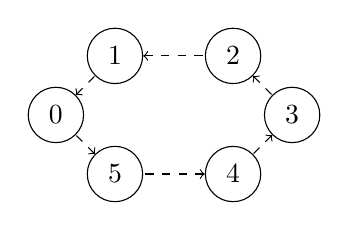
\begin{tikzpicture}[scale=0.75]
			\tikzstyle{vertex}  = [circle, minimum size=20pt, inner sep=0pt, draw=black, fill=white]
			
%			\draw[step=1cm, gray!50] (-2.4,-2.4) grid (2.4,3.4);

			\node[vertex] (dep) at (0, 0) {$0$};
			
			\foreach \text/\x/\y in {1/1/1, 2/3/1, 3/4/0, 4/3/-1, 5/1/-1}
				\node[vertex] (\text) at (\x, \y) {$\text$};
			
			\foreach \from/\to in {}
				\path[<-] (\to) edge node [swap] {} (\from);
			
			\foreach \from/\to in {dep/1, 1/2, 2/3, 3/4, 4/5, 5/dep}
				\path[<-, dashed] (\from) edge node {} (\to);	

		\end{tikzpicture}		
		
	}
		
	\caption{Operadores intra-ruta de generación de vecindades.}
	\label{Oper-intra}
\end{figure}

\subsection{Búsqueda descendente en vecindades variables (VND)} \label{sect:implementacion-vnd}

El algoritmo de búsqueda descendente en vecindades variables propuesto en \cite{VNDimp} se encarga de cambiar sistemáticamente la vecindad actual de manera determinística.
 
El algoritmo propuesto utiliza un conjunto de once operadores de vecindad. Sólo se admiten modificaciones factibles, es decir, aquellas que no violen la condición de carga permitida en un vehículo. De los operadores utilizados seis hacen modificaciones inter-ruta y el resto intra-ruta.

A continuación se muestran los operadores inter-ruta utilizados. Los operadores se utilizan dentro del algoritmo en el mismo orden en el que están descritos:

\begin{itemize}

\item \textbf{Shift(1,0):} Relocaliza un cliente de una ruta $r_i$ a una ruta $r_j$.

\item \textbf{Crossover:} Descrito anteriormente en \textbf{Sección~\ref{sect:implementacion-busquedalocal}}.

\item \textbf{Swap(1,1):} Permuta dos clientes de dos rutas distintas.

\item \textbf{Shift(2,0):} Relocaliza dos clientes consecutivos de una ruta $r_i$ a una ruta $r_j$.

\item \textbf{Swap(2,1):} Permuta dos clientes consecutivos de una ruta con un cliente de otra ruta.

\item \textbf{Swap(2,2):} Permuta dos clientes consecutivos de una ruta con dos clientes consecutivos de otra ruta.

\end{itemize}

En caso de mejorar la solución actual, se utilizan operadores capaces de mejorar la calidad de las rutas mo\-di\-fi\-ca\-das que contribuyeron a reducir el costo de la solución. Para ello se utilizan los siguientes operadores intra-ruta descritos anteriormente en \textbf{Sección~\ref{sect:implementacion-busquedalocal}}:

\begin{itemize}
\item \textbf{Or-opt:} Selecciona aleatoriamente alguno de los siguientes operadores: Or-opt(1), Or-opt(2) ó Or-opt(3).
\item \textbf{Or-opt(1):} Relocaliza un cliente en su misma ruta.
\item \textbf{Or-opt(2):} Relocaliza dos clientes consecutivos en su misma ruta.
\item \textbf{Or-opt(3):} Relocaliza tres clientes consecutivos en su misma ruta.
\item \textbf{2-opt: } Descrito anteriormente en \textbf{Sección~\ref{sect:implementacion-busquedalocal}}.
\item \textbf{Reverse: } Descrito anteriormente en \textbf{Sección~\ref{sect:implementacion-busquedalocal}}.
\item \textbf{Swap: } Permuta dos clientes de una misma ruta.
\end{itemize}

El pseudocódigo general de VND se puede ver en el \textbf{Apéndice~\ref{chap:apendiceA}}, \textbf{Algoritmo~\ref{alg:VND}}.

\subsection{Mecanismos de Perturbación}
\label{sect:perturbacion}

Con el propósito de cambiar una solución se utiliza una perturbación. Es importante destacar que todas las per\-tur\-ba\-cio\-nes realizan cambios factibles dentro de las soluciones. Los operadores implementados fueron los siguientes:\\

\begin{itemize}
\item \textbf{Ejection Chain:} Aplicado en  \cite{PertEC} para una versión clásica de VRP, funciona de la sieguiente manera. Un cliente de una ruta $r_i$ se transfiere a una ruta $r_j$. Un cliente de la ruta $r_j$ se transfiere a la ruta $r_k$ y así sucesivamente. El movimiento termina cuando un cliente de la última ruta transfiere a un cliente a la primera ruta. Los clientes son escogidos aleatoriamente.

\item \textbf{Double-Swap:} Realiza dos operaciones secuenciales y factibles de Swap con dos clientes seleccionados alea\-to\-ria\-men\-te. 

\item \textbf{Double-Bridge:} Introducido en \cite{PertDB}, esta perturbación fue desarrollada originalmente para TSP\footnote{TSP: Traveling Salesman Problem}. Con\-sis\-te en eliminar cuatro arcos de una ruta y agregar cuatro nuevos. Se aplica aleatoriamente en solo algunas de las rutas.
\end{itemize}


\section{Metaheurísticas híbridas} \label{sect:implementacion-heuristicas-hibridas}

En esta sección se presentan los detalles de implementación de las seis metaheurísticas híbridas implementadas en este trabajo.

\subsection{Búsqueda Local Iterada con Vecindades Variables Modificada (ILS-VND-M)} \label{sect:implementacion-ils}

El algoritmo búsqueda local iterada con vecindades variables (ILS-VND por sus siglas en inglés de \emph{Iterated Local Search with Variable Neightborhood Descent}) basado en \cite{ils-vnd} trabaja de la siguiente manera. Tiene un procedimiento principal, el cual se ejecuta un número máximo de iteraciones $n$, en donde la solución inicial es generada por una heurística greedy. La misma usa como parámetros un factor $y$ para su función de costo y un entero $k$ que determina la cantidad de rutas de la solución. \\

La solución es mejorada por un procedimiento basado en la metaheurística ILS, el cual consta de dos partes principales, un método de mejoramiento y una perturbación de la solución. Este procedimiento consta de un criterio de parada en el cual no pueden transcurrir $LS$ iteraciones sin que se encuentre una mejor solución que la encontrada hasta el momento dentro del procedimiento. De encontrar una mejor solución el iterador de criterio de parada se reinicia. Al salir de este procedimiento se compara la mejor solución obtenida con la mejor solución encontrada en iteraciones anteriores del procedimiento principal.

La solución inicial se basa en el algoritmo de inserción descrito en la \textbf{Sección~\ref{sect:implementacion-algoritmos-iniciales}}. El método de mejoramiento es realizado por la metaheurística VND descrita en la \textbf{Sección~\ref{sect:implementacion-vnd}}. Por último, para la perturbación se proponen tres mecanismos distintos, \textit{Ejection Chain}, \textit{Double Swap} y \textit{Double Bridge} respectivamente.Cada vez que se invoque a la función de perturbación se escoge alguno de ellos aleatoriamente. Cada uno de estos mecanismos se encuentran descritos en la \textbf{Sección~\ref{sect:perturbacion}}.\\

El pseudocódigo general de ILS-VND-M se puede ver en el \textbf{Apéndice~\ref{chap:apendiceA}}, \textbf{Algoritmo~\ref{alg:ILS-VND-M}}.

\subsubsection*{Variantes de Implementación}

El algoritmo ILS-VND-M no presenta diferencias con respecto a la implementación propuesta en  \cite{ils-vnd}.

\subsubsection*{Parámetros}

Las siguientes variables se establecieron como parámetros de ILS-VND-M por la influencia que pueden causar en los resultados finales:


\begin{table}[ht]
\centering
\small
\caption{Parámetros de ILS-VND-M}
\begin{tabular}{l||p{15cm}}
\hline\hline\\
\textbf{n} & Número de iteraciones máximas en el procedimiento principal.\\ [0.7ex]\cline{2-2}\\
\textbf{LS} & Número de iteraciones máximas sin mejorías dentro de la sección del método de mejoramiento y perturbación de la solución. \\ 
[0.7ex]\cline{2-2}\\
\textbf{y} & Factor que influye en la función de costo del algoritmo de inserción para la solución inicial.\\
\\ \hline\hline
\end{tabular}
\label{table:param-ils}
\end{table}



\subsection{Búsqueda Tabú Guiada Modificada (GTS-M)} \label{sect:implementacion-gts}


La búsqueda tabú guiada (GTS por sus siglas en inglés de \emph{Guided Tabu Search}) es una fusión o hibridación de dos metaheurísticas bien conocidas como lo son \emph{Búsqueda Tabú (TS)} y \emph{Búsqueda Local Guiada (GLS)}, implementada basándose en \cite{gts}. Estas dos metaheurísticas han probado ser efectivas para resolver VRP y sus variantes según \cite{gts1}, \cite{gts2}, \cite{gts3}, \cite{gts4}, \cite{gts5}. 

La solución inicial para GTS-M se obtiene del algoritmo de construcción basado en ahorro de costos, \textbf{ver Sección \ref{sect:implementacion-algoritmos-iniciales}}. 

Una vez creada la solución inicial, ésta es mejorada utilizando la hibridación TS-GLS. En orden de explorar el espacio de soluciones, la solución es modificada subsecuentemente como todo método de búsqueda local. Para esto cuatro tipos de movimientos intra-ruta e inter-ruta son utilizados mediante el uso de siete operadores. Adi\-cio\-nal\-men\-te, una búsqueda descendiente en vecindades variables es realizada  según lo especificado previamente en la \textbf{Sección \ref{sect:implementacion-vnd}}.

Los movimientos a ejecutar son los siguientes:

\begin{itemize}
\item \textbf{Movimiento exchange.} Operadores: Swap de dos clientes intra-ruta, Swap de dos clientes inter-ruta.
\item \textbf{Movimiento relocate.} Operadores: Or-opt intra-ruta de un cliente, Shift inter-ruta de un cliente.
\item \textbf{Movimiento interchange 1.} Operadores: 2-opt intra-ruta, Crossover inter-ruta.
\item \textbf{Movimiento interchange 2.} Operador: Interchange inter-ruta.
\end{itemize}

Para limitar el tiempo de cómputo tomado por los movimientos mencionados, un esquema de reducción de vecindad es aplicado. Para cada cliente $i$ se define como $avg_i$ el costo promedio de todos los arcos adyacentes a $i$, y se define la vecindad $NV_i$ como todos los clientes adyacentes a $i$ cuyo costo sea menor a $avg_i$. De esta manera, se permite la creación de un nuevo arco desde $j$ a $k$ sólo si $k \in NV_j$.\\


\subsubsection*{Desarrollo de la metaheurística}

Se genera la solución inicial mediante el algoritmo de construcción. En cada iteración de GTS-M se selecciona uno de los cuatro movimientos mencionados de manera probabilística. Realizando pruebas empíricas se determinó que los movimientos \emph{exchange} y \emph{relocate} consumen poco tiempo computacional y consiguen reducir más el valor de la función objetivo en comparación con los movimientos \emph{interchange 1} e \emph{interchange 2}. Sin embargo se determinó que estas últimas influyen más en la exploración, ya que diversifican de gran manera las soluciones, haciéndolas imprescindibles. Por lo tanto se decidió establecer una probabilidad de selección de $\frac{1}{3}$ para \emph{exchange} y \emph{relocate}, mientras que a \emph{interchange 1} e \emph{interchange 2} se le otorgó una probabilidad de $\frac{1}{6}$.

El movimiento escogido se efectúa, se realiza primeramente el operador intra-ruta especificado para realizar el mejor cambio posible dentro de una ruta entre cada una de las rutas, para luego realizar el operador inter-ruta, de manera de realizar el mejor cambio posible entre rutas. Si no se encuentra ninguna solución que mejore la solución actual, se procede a realizar VND.
Mediante TS, la nueva solución es escogida sólo si no se encuentra en la lista tabú o ha superado el criterio de aspiración (que la solución sea la mejor encontrada hasta el momento). Seguidamente todos los movimientos reversos (aquellos movimientos que lleven a la solución actual) son incluídos en la \emph{lista tabú} por \emph{tabu} iteraciones. La lista tabú se implementó como una lista circular doblemente enlazada de tamaño \emph{tabú}, utilizada como cola. De esta manera se simplifica la adición o sustracción de nuevos movimientos en la lista tabú realizándolos en tiempo constante.

El procedimiento anterior es continuamente coordinado por GLS penalizando el arco $i-j$ perteneciente a la solución actual que maximice la siguiente función de utilidad:

\begin{equation}
U(i,j) = \frac{c_{ij}/avg_{ij}}{1 + p_{ij}}
\end{equation}

Donde $p_{ij}$ es el número de veces que el arco $i-j$ ha sido penalizado, $avg_{ij}$ representa el costo medio de los arcos adyacentes a $i$ y los adyacentes a $j$ y $c_{ij}$ representa el costo entre los clientes $i$ y $j$.\\

Finalmente, GTS-M termina luego que cumplir \emph{mni} iteraciones sin lograr ninguna mejoría a la solución actual.\\

El pseudocódigo general de GTS-M se puede ver en el \textbf{Apéndice~\ref{chap:apendiceA}}, \textbf{Algoritmo~\ref{alg:GTS}}.

\subsubsection*{Variantes de Implementación}

El GTS-M implementado tiene varias diferencias con respeto al propuesto por \cite{gts}. Al momento de se\-leccio\-nar un movimiento, éste  se selecciona de manera probabilística beneficiando a aquellos que consumen menos tiempo de cómputo, mientras que en el trabajo referenciado se selecciona de manera indefinida. Además, GTS-M al momento de realizar el movimiento ya seleccionado, aplica VND si el movimiento no mejora la solución actual, mientras que en el trabajo referenciado se crea una nueva iteración.\\

\subsubsection*{Parámetros}

Las variables en la \textbf{Tabla~\ref{table:param-gts}} se establecieron como parámetros de GTS-M por la influencia que pueden causar en los resultados finales.

\begin{table}[ht]
\centering
\small
\caption{Parámetros de GTS-M}
\begin{tabular}{l||p{15cm}}
\hline\hline\\
\textbf{mni} & Número de iteraciones máximas sin mejorías\\ [0.7ex]\cline{2-2}\\
\textbf{lambda1} & Valor utilizado en el algoritmo de construcción de la solución inicial que controla
					la importancia relativa entre insertar un cliente en una nueva ruta o no. Siendo los valores cercanos a $0$ una alta probabilidad de
				 	insertar el cliente en la ruta escogida, y los valores cercanos a $1$ una baja probabilidad
				 	de insertarla\\ [0.7ex]\cline{2-2}\\
\textbf{lambda2} & Valor utilizado en GLS que controla la interacción entre exploración del espacio de soluciones
					y explotación de la solución actual. Siendo los valores cercanos a 0 una inclinación por la
					explotación de la solución actual, y los valores cercanos a 1 una inclinación por la exploración
					del espacio de soluciones\\ [0.7ex]\cline{2-2}\\
\textbf{tabu} & Tamaño de la lista tabú o número de iteraciones que un movimiento es declarado tabú\\
\\ \hline\hline
\end{tabular}
\label{table:param-gts}
\end{table}

\subsection{Sistema de Hormigas Modificado (AS-M)} \label{sect:implementacion-aco}

Sistema de hormigas (AS por sus siglas en inglés de \emph{Ant System}) es una metaheurística de tipo ACO que busca minimizar el costo de las soluciones fundamentándose en el intercambio de información de poblaciones realizando reforzamiento de feromonas. Fue implementada basándose en \cite{maco}.

La metaheurística AS-M genera una solución inicial factible mediante el algoritmo de vecino más cercano (ver \textbf{Sección \ref{sect:implementacion-algoritmos-iniciales}}) para dirigir a las hormigas en la construcción de las soluciones. En los arcos de esta solución  se deposita una cantidad inicial fija de feromonas.
Una vez hecho esto se ubican $l$ hormigas, donde $l$ es el número de clientes del problema VRPSPD. Cada hormiga construye su propia solución independientemente, basándose en la atractividad de los clientes, depositando feromonas en todos los arcos por los que se desplaza. Luego de que todas las hormigas crean sus soluciones, se aplica VND a cada solución con el propósito de mejorarlas y se guarda la mejor solución encontrada. El procedimiento anterior es repetido $n$ iteraciones y la mejor solución encontrada se reporta.

\subsubsection*{Desarrollo de la metaheurística}

Se crea la solución inicial y se deposita una cantidad inicial $\tau_0$ de feromonas en cada arco perteneciente a la solución. Se ha observado en la literatura \cite{aco-pheromone} que $\tau_0 = 1/lL_0$ impulsa a la metaheurística a construir posteriormente buenas soluciones. $l$ es el número de clientes del problema y $L_0$ es el costo de la solución inicial. Posteriormente, la visibilidad $\eta_{ij}$, entre cada par de clientes es calculada basándose en la siguiente ecuación:

\begin{equation}
\eta_{ij} = \frac{c_{i0} + c_{0j} - c_{ij}}{c_{ij}}
\end{equation}

De esta manera se beneficia el hecho de que dos clientes cercanos, y a su vez lejanos del depósito, estén en la misma ruta y no en rutas distintas.\\

La iteración se inicia colocando una hormiga en cada uno de los clientes. Cada una construye su propia solución basándose en la atractividad de los próximos clientes. Se crea una nueva ruta vacía y se coloca el depósito como el primer cliente visitado, seguido por el cliente de la posición de la hormiga. Para cada hormiga $k$, se crea, a medida que la hormiga construye su solución, una vecindad $N_i^k$ de cada cliente $i$ que contiene los clientes no visitados por la hormiga $k$ que no violan las restricciones del problema. Si $N_i^k$ se encuentra vacío, la hormiga regresa al depósito finalizando esa ruta y comenzando otra desde el depósito. El procedimiento anterior se repite hasta que todos los clientes sean visitados y cada una de las hormigas finalice la construcción de sus soluciones.

La selección del próximo cliente a visitar está basada en el valor de atractividad entre el cliente actual y los clientes en su vecindad. La atractividad entre el cliente $i$ y el $j$ está definida como $\phi_{ij}$ = $(\tau_{ij})^\alpha(\eta_{ij})^\beta$. Donde $\tau_{ij}$ es la cantidad de feromonas en el arco $i$-$j$, $\alpha$ y $\beta$ son parámetros positivos para controlar la importancia relativa entre el peso de las feromonas y el peso de la información heurística de la visibilidad en la atractividad. 

La hormiga $k$ localizada en el cliente $i$ puede visitar su cliente más favorable o seleccionar uno probabilísticamente, dependiendo de la siguiente regla: 

\begin{equation}
 p_i^k =
  \begin{cases}
   j \text{ }|\text{ } Max\{\phi_{ij}\} 	& \text{si } q_r \leqslant q\\
   j' 					& \text{en otro caso}
  \end{cases}
\end{equation}

donde $q$ es un parámetro que controla la importancia relativa entre la exploración y la explotación, y $q_r$ es una variable aleatoria distribuida uniformemente tal que $q_r \in [0,1]$.
En el caso en que la hormiga no se dirija hacia el cliente más atractivo, probabilísticamente se seleciona otro cliente basándose en su atractividad, utilizando la siguiente distribución de probabilidad:

\begin{equation}
 j' =
  \begin{cases}
   j \text{ }|\text{ } \frac{\phi_{ij}}{\sum\limits_{l\in N_{l}^{k}}\phi_{il}} 	& \text{si } j\in N_{l}^{k}\\
   0 					& \text{en otro caso}
  \end{cases}
\end{equation}

Luego de que una hormiga construya sus rutas, se aplica VND a la solución con el fin de mejorarla.\\


Posteriormente de que todas las hormigas construyan sus soluciones, se realiza la evaporación de las feromonas y el reforzamiento de caminos con nuevas feromonas, ordenando todas las hormigas ascendentemente, según la calidad de su solución encontrada (según el costo total). De esta manera, si un arco $i$-$j$ es utilizado por $r$-mejor hormiga, las feromonas en ese arco son incrementadas en:

\begin{equation}
\Delta\tau_{ij}^r = \frac{(\lambda - r + 1)}{L_r}
\end{equation}

donde $L_r$ es el costo de la solución construida por la $r$-mejor hormiga y $\lambda$ es el número de hormigas. Por lo tanto la actualización de feromonas se realiza de la siguiente manera:

\begin{equation}
\tau_{ij}^r = (1 - \rho)\tau_{ij} + \sum_{r=1}^{\lambda}\Delta\tau_{ij}^r
\end{equation}

donde $\rho$ representa la rápidez de evaporación de feromonas. Finalmente, se registra la mejor solución obtenida hasta el momento y se finaliza la iteración.\\

El pseudocódigo general de AS-M se puede ver en el \textbf{Apéndice~\ref{chap:apendiceA}}, \textbf{Algoritmo~\ref{alg:MACO}}.

\subsubsection*{Variantes de Implementación}

AS-M se diferencia de \cite{maco} en que la mejora de la solución se realiza utilizando VND en lugar de búsqueda local.

\subsubsection*{Parámetros}

Las variables en la \textbf{Tabla~\ref{table:param-aco}} se establecieron como parámetros de AS-M por la influencia que pueden causar en los resultados finales.

\begin{table}[ht]
\centering
\small
\caption{Parámetros de AS-M}
\begin{tabular}{l||p{15cm}}
\hline\hline\\
\textbf{n} & Número de iteraciones\\ [0.7ex]\cline{2-2}\\
\textbf{alpha} & Variable que define la importancia de la feromona en la atractividad de un cliente\\ [0.7ex]\cline{2-2}\\
\textbf{beta} & Variable que define la importancia de la visibilidad en la atractividad de un cliente\\ [0.7ex]\cline{2-2}\\
\textbf{q} & Variable que define la importancia relativa entre exploración y explotación de la metaheurística \\ [0.7ex]\cline{2-2}\\
\textbf{ro} & Rapidez de evaporación de las feromonas\\
\\ \hline\hline
\end{tabular}
\label{table:param-aco}
\end{table}



\subsection{Busqueda en Dispersión Modificada (SS-M)} \label{sect:implementacion-SS}

La búsqueda en dispersión (SS por sus siglas en inglés de \emph{Scatter Search}) está basado en \cite{SCAimp} y funciona de la siguiente manera. Comienza al crear un pool de soluciones diversas con el método de diversificación y actualizar el Refset. 

Luego realiza un proceso iterativo donde se escoge subconjuntos de soluciones pertenecientes al Refset y a\-pli\-ca con estos el método de combinación. Todas las soluciones derivadas de este método son sujetas al método de mejoramiento y luego son utilizadas para actualizar el Refset. Este proceso iterativo se mantiene hasta que en alguna iteración ninguna nueva solución sea admitida en el Refset. Finalmente, se aplica el VND  descrito en la \textbf{sección~\ref{sect:implementacion-vnd}}, a cada una de las soluciones que le pertenecen al Refset y se selecciona la mejor.\\

Las soluciones del Refset no son cambiadas hasta que todas las combinaciones son realizadas.\\ 

Sea $P$ un conjunto de soluciones diversas creado por el método de diversificación   y $Psize$ el tamaño de la población $P$. $Refset$ es el conjunto de referencia y su tamaño es $b$. El conjunto de referencia contiene dos sub\-con\-jun\-tos, uno con $b_{1}$ soluciones de calidad $Refset_{1}$ y otro con $b_{2}$ soluciones diversas $Refset_{2}$, por lo tanto $b = b_{1} + b_{2}$. Las soluciones dentro del conjunto de referencia son representadas por $Refset^{j}$, para $j={1,...,b}$. $NewSubset$ es el subconjunto de soluciones escogidas del $Refset$ y el $Pool$ el conjunto de soluciones generadas por el método de combinación.\\

A continuación se describen cada uno de los métodos de mayor importancia dentro de la metaheurística.

\subsubsection*{Método de Generación Diversificada}

 Se generan \textit{Psize} soluciones a través de un algoritmo ambicioso de construcción aleatoria descrito en la \textbf{sección~\ref{sect:implementacion-algoritmos-iniciales}}.
 
\subsubsection*{Método de Mejoramiento}

Se utilizan vecindades variables como algoritmo de mejoramiento para las rutas. Entre los operadores inter-ruta utilizados se encuentran, Shift(1,0), Crossover, Swap(1,1). Entre los operadores intra-ruta utilizados se encuentran Or-opt(1), Swap(1,1) y 2-opt. Todos descritos anteriormente en \textbf{Sección~\ref{sect:implementacion-vnd}}.

\subsubsection*{Método de Actualización del Refset}

Se escogen de las $Psize$ soluciones del conjunto $P$ las $b_{1}$ so\-lu\-cio\-nes que tengan el mejor costo. Éstas se añaden al $Refset$ y son eliminadas de $P$.\\ 

Luego adicionalmente se escogen $b_{2}$ soluciones de mayor diversidad y son añadidas al $Refset$. Para medir la diversidad, la distancia entre dos soluciones, $s_{1}$ y $s_{2}$,   debe de ser calculada. Para realizar esto, se crea una matriz cuadrada llamada ClientCount de tamaño $r*r$, donde $r$ es el máximo número de rutas entre $s_{1}$ y $s_2$. A continuación se procede a llenar la matriz de tal manera que contenga el número de clientes comunes en la ruta $i$ de la solución $s_1$ y la ruta $j$ de la solución $s_{2}$. Una vez realizado esto se  busca el mayor elemento de la matriz y se suma con el acumulado hasta el momento, para luego borrar la fila y la columna correspondiente a la posición del elemento, este proceso se repite hasta que la matriz no pueda seguir siendo reducida. Por último se resta este valor al número total de clientes, este cálculo da como resultado la distancia entre dos soluciones.\\

Para ilustrar esto considere las siguientes soluciones:\\

$s_{1}$: (3,7)(4,5,8,6)(10,2,9,1)
$s_{2}$: (7,9,6,8,5)(1,2,3,4,10)\\

El valor de r es 3 y la matriz ClientCount resultante tiene la siguiente forma:\\

\begin{tabular}{|c|c|c|c|}
\hline \rule[-2ex]{0pt}{5.5ex} { } & $s_{21}$ & $s_{22}$ & $s_{23}$ \\ 
\hline \rule[-2ex]{0pt}{5.5ex} $s_{11}$ & 1 & 1 & 0 \\ 
\hline \rule[-2ex]{0pt}{5.5ex} $s_{12}$ & 3 & 1 & 0 \\ 
\hline \rule[-2ex]{0pt}{5.5ex} $s_{13}$ & 1 & 3 & 0 \\ 
\hline 
\end{tabular}\\\\ 



Luego de seleccionar los elementos $(s_{13},s_{22})$ y $(s_{12},s_{21})$ y eliminar en cualquier orden sus columnas y filas co\-rres\-pon\-dien\-tes queda solamente el elemento $(s_{11},s_{23})$. El resultado de la suma de los mayores elementos es 6, lo cual daría como resultado de la distancia lo siguiente:\\

\begin{equation}
\# ClientesTotal - \# Acumulado = distancia 
\end{equation}
\\ 
es decir:
\\
\begin{center}
$10 – 6 = 4$
\end{center}

El método calcula la distancia entre una solución de $P$ y todas las que se encuentren en $Refset$, aquella que tenga la mayor distancia acumulada es eliminada de $P$ y agregada en $Refset$. Este proceso se repite hasta que se seleccionen $b_{2}$ soluciones para que el $Refset$ tenga $b$ soluciones, $b_{1}$ escogidas por calidad y $b_{2}$ por diversidad.

\subsubsection*{Método de Combinación}

El método de combinación opera en un par de soluciones que son tomadas del Refset con la lista de soluciones generadas por el método de generación de subconjuntos. La lista de pares de soluciones es tal, que al menos una de ellas es considerada una solución nueva, es decir, fue admitida en el $Refset$ durante la última iteración.  El método comienza por comparar un par de rutas entre dos soluciones, luego extrae los clientes semejantes, dejando así una nueva solución parcial.\\
 
Para crear una solución completa, se insertan los clientes que aun no han sido asignados en las existentes rutas parciales. La inserción es ambiciosa, tratando de disminuir la distancia incremental de añadir un cliente no asignado a la ruta existente. Si el cliente no puede ser asignado a ninguna de las rutas, se crea una ruta nueva en donde será colocado.\\

En la \textbf{figura~\ref{SCA:comb}} se puede observar el funcionamiento del mismo. El grafo \textbf{(a)} y el grafo \textbf{(b)} representan  las soluciones que serán combinadas. El grafo \textbf{(c)} muestra la solución incompleta resultante de obtener los clientes comunes entre ambas soluciones. Por último el grafo \textbf{(d)} representa la solución final resultante de la inserción de los clientes restantes.


\begin{figure}[h]
	\begin{center}
	\begin{tabular}{@{}l@{}}
		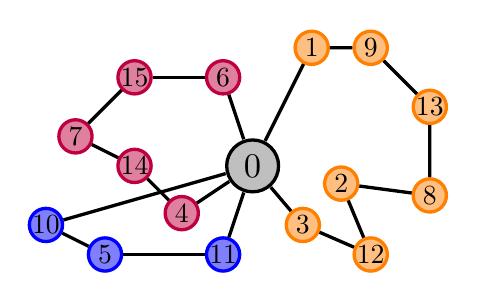
\begin{tikzpicture}[scale=0.75, auto, very thick]
			\tikzstyle{vertex}   = [circle, minimum size=15pt, inner sep=0pt, draw=black, fill=black!25, scale=1.25]
			\tikzstyle{vertexA}  = [circle, minimum size=12pt, inner sep=0pt, draw=purple, fill=purple!50]
			\tikzstyle{vertexB}  = [circle, minimum size=12pt, inner sep=0pt, draw=blue, fill=blue!50]
			\tikzstyle{vertexC}  = [circle, minimum size=12pt, inner sep=0pt, draw=orange, fill=orange!50]
			
%			\draw[step=1cm, gray!50] (-2.4,-2.4) grid (2.4,3.4);

			\node[vertex] (dep) at (0, 0) {$0$};
			
			\foreach \text/\x/\y/\styl in {9/2/2/C,1/1/2/C,6/-0.5/1.5/A,15/-2/1.5/A, 7/-3/0.5/A, 14/-2/0/A, 4/-1.2/-0.8/A, 10/-3.5/-1/B, 5/-2.5/-1.5/B, 11/-0.5/-1.5/B, 13/3/1/C, 2/1.5/-0.3/C, 8/3/-0.5/C, 12/2/-1.5/C, 3/0.85/-1/C}
				\node[vertex\styl] (\text) at (\x, \y) {$\text$};
			
			\foreach \from/\to in {dep/1, 1/9, 9/13, 13/8, 8/2, 2/12, 12/3, 3/dep, dep/10, 10/5, 5/11, 11/dep, dep/6, 6/15, 15/7, 7/14, 14/4, 4/dep}
				\path[-] (\to) edge node [swap] {} (\from);

		\end{tikzpicture}
    (a)
\hspace{10mm}
    (b) 
		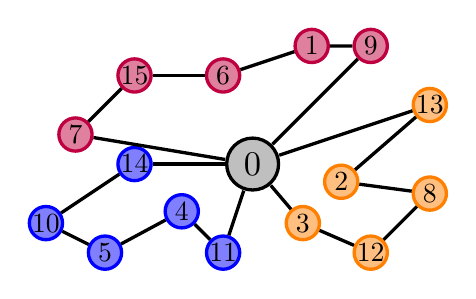
\begin{tikzpicture}[scale=0.75, auto, very thick, ]
			\tikzstyle{vertex}   = [circle, minimum size=15pt, inner sep=0pt, draw=black, fill=black!25, scale=1.25]
			\tikzstyle{vertexA}  = [circle, minimum size=12pt, inner sep=0pt, draw=purple, fill=purple!50]
			\tikzstyle{vertexB}  = [circle, minimum size=12pt, inner sep=0pt, draw=blue, fill=blue!50]
			\tikzstyle{vertexC}  = [circle, minimum size=12pt, inner sep=0pt, draw=orange, fill=orange!50]
			
%			\draw[step=1cm, gray!50] (-2.4,-2.4) grid (2.4,3.4);

			\node[vertex] (dep) at (0, 0) {$0$};
			
			\foreach \text/\x/\y/\styl in {9/2/2/A,1/1/2/A,6/-0.5/1.5/A,15/-2/1.5/A, 7/-3/0.5/A, 14/-2/0/B, 4/-1.2/-0.8/B, 10/-3.5/-1/B, 5/-2.5/-1.5/B, 11/-0.5/-1.5/B, 13/3/1/C, 2/1.5/-0.3/C, 8/3/-0.5/C, 12/2/-1.5/C, 3/0.85/-1/C}
				\node[vertex\styl] (\text) at (\x, \y) {$\text$};
			
			\foreach \from/\to in {dep/9, 9/1, 1/6, 6/15, 15/7, 7/dep, dep/14, 14/10, 10/5, 5/4, 4/11, 11/dep, dep/13, 13/2, 2/8, 8/12, 12/3, 3/dep}
				\path[-] (\to) edge node [swap] {} (\from);

		\end{tikzpicture}\\\\

		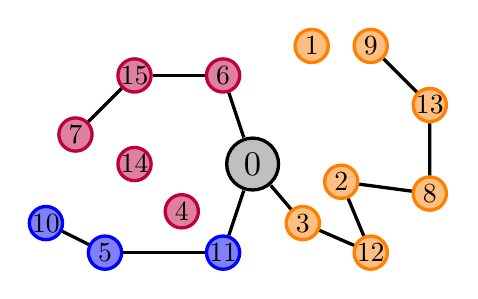
\begin{tikzpicture}[scale=0.75, auto, very thick]
			\tikzstyle{vertex}   = [circle, minimum size=15pt, inner sep=0pt, draw=black, fill=black!25, scale=1.25]
			\tikzstyle{vertexA}  = [circle, minimum size=12pt, inner sep=0pt, draw=purple, fill=purple!50]
			\tikzstyle{vertexB}  = [circle, minimum size=12pt, inner sep=0pt, draw=blue, fill=blue!50]
			\tikzstyle{vertexC}  = [circle, minimum size=12pt, inner sep=0pt, draw=orange, fill=orange!50]
			
%			\draw[step=1cm, gray!50] (-2.4,-2.4) grid (2.4,3.4);

			\node[vertex] (dep) at (0, 0) {$0$};
			
			\foreach \text/\x/\y/\styl in {9/2/2/C,1/1/2/C,6/-0.5/1.5/A,15/-2/1.5/A, 7/-3/0.5/A, 14/-2/0/A, 4/-1.2/-0.8/A, 10/-3.5/-1/B, 5/-2.5/-1.5/B, 11/-0.5/-1.5/B, 13/3/1/C, 2/1.5/-0.3/C, 8/3/-0.5/C, 12/2/-1.5/C, 3/0.85/-1/C}
				\node[vertex\styl] (\text) at (\x, \y) {$\text$};
			
			\foreach \from/\to in { 9/13, 13/8, 8/2, 2/12, 12/3, 3/dep, 10/5, 5/11, 11/dep, dep/6, 6/15, 15/7}
				\path[-] (\to) edge node [swap] {} (\from);

		\end{tikzpicture}
    (c)
\hspace{10mm}
    (d) 
		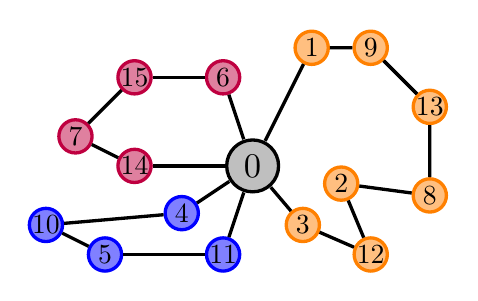
\begin{tikzpicture}[scale=0.75, auto, very thick]
			\tikzstyle{vertex}   = [circle, minimum size=15pt, inner sep=0pt, draw=black, fill=black!25, scale=1.25]
			\tikzstyle{vertexA}  = [circle, minimum size=12pt, inner sep=0pt, draw=purple, fill=purple!50]
			\tikzstyle{vertexB}  = [circle, minimum size=12pt, inner sep=0pt, draw=blue, fill=blue!50]
			\tikzstyle{vertexC}  = [circle, minimum size=12pt, inner sep=0pt, draw=orange, fill=orange!50]
			
%			\draw[step=1cm, gray!50] (-2.4,-2.4) grid (2.4,3.4);

			\node[vertex] (dep) at (0, 0) {$0$};
			
			\foreach \text/\x/\y/\styl in {9/2/2/C,1/1/2/C,6/-0.5/1.5/A,15/-2/1.5/A, 7/-3/0.5/A, 14/-2/0/A, 4/-1.2/-0.8/B, 10/-3.5/-1/B, 5/-2.5/-1.5/B, 11/-0.5/-1.5/B, 13/3/1/C, 2/1.5/-0.3/C, 8/3/-0.5/C, 12/2/-1.5/C, 3/0.85/-1/C}
				\node[vertex\styl] (\text) at (\x, \y) {$\text$};
			
			\foreach \from/\to in { 9/13, 13/8, 8/2, 2/12, 12/3, 3/dep, 10/5, 5/11, 11/dep, dep/6, 6/15, 15/7, 7/14, 14/dep, 10/4, 4/dep, dep/1, 1/9, 9/13}
				\path[-] (\to) edge node [swap] {} (\from);

		\end{tikzpicture}


	\end{tabular}

	\end{center}
	\caption[Ilustración del método de combinación]{\textsl{Ilustración del método de combinación}}
	\label{SCA:comb}
\end{figure}

El pseudocódigo general de SS-M se puede ver en el \textbf{Apéndice~\ref{chap:apendiceA}}, \textbf{Algoritmo~\ref{alg:SCA-M}}.   

\subsubsection*{Variantes de Implementación}

El SS-M implementado tiene una diferencia con el planteado en el artículo  base \cite{SCAimp} en el método de combinación . En \cite{SCAimp} se realiza la mejor inserción posible de un solo cliente escogido arbitrariamente, mientras que el mecanismo de inserción utilizado en SS-M se escoge entre todos los clientes no asignados aquel cliente que dé el menor costo añadido a la solución parcial.

\subsubsection*{Parámetros}

Las siguientes variables se establecieron como parámetros de SS-M por la influencia que pueden causar en los resultados finales:

\begin{table}[ht]
\centering
\small
\caption{Parámetros de SS-M}
\begin{tabular}{l||p{15cm}}
\hline\hline\\
\textbf{n} & Tamaño del \textit{Pool}.\\ 
[0.7ex]\cline{2-2}\\
\textbf{b} & Tamaño del Refset.\\ 
[0.7ex]\cline{2-2}\\
\textbf{y} & Variable que define la función de costo del método de diversificación.\\
\\ \hline\hline
\end{tabular}
\label{table:param-ss}
\end{table}


\subsection{Algoritmo Genético Modificado (GA-M)} \label{implementacion-GA-M}

El algoritmo genético (GA por sus siglas en inglés de \emph{Genetic Algorithm}) basado en \cite{IGAimp} empieza por obtener una población inicial, es decir, la primera generación. Se asume que la población inicial contiene una cantidad $p$ de individuos, donde $p$ es un entero. 

Luego de calcular el valor del fitness\footnote{Ver \textbf{Sección~\ref{subsect:GA}}} para cada uno de los individuos de la población inicial, comienza el proceso de selección de dos individuos aleatoriamente, este proceso se repite $p/2$ veces. El criterio de cruce consiste en tomar un entero aleatorio y compararlo con $cprob$, si este resulta ser menor que $cprob$ entonces se procede a aplicar el operador de cruce para producir dos nuevos hijos, de lo contrario continua el proceso de selección de los padres. Subsecuentemente se procede con el proceso de mutación de estos nuevos individuos si cumplen con el criterio, el cual consiste en tomar un entero aleatorio y compararlo con $mprob$, si este resulta ser menor que $mprob$ entonces se procede a aplicar la mutación. Finalmente se calcula para cada hijo su valor de fitness. Para obtener la nueva generación se mantiene el criterio de \textit{"steady-state"}. Luego de alcanzar el número máximo de iteraciones denotado como $n$ el algoritmo pasa la solución a un proceso de mejoramiento logrado con la metaheurística VND  descrita en la \textbf{Sección~\ref{sect:implementacion-vnd}}, a cada una de las soluciones de la población y selecciona la mejor.\\ 

\subsubsection*{Solución Inicial y Fitness}

La solución inicial es obtenida con el algoritmo ambicioso de construcción aleatoria descrito en la \textbf{sección~\ref{sect:implementacion-algoritmos-iniciales}}, este proceso se realiza hasta que el número de soluciones alcance $p$.\\

$k_{max}$ es la cantidad máxima de rutas permitidas en una solución, $r$ es la cantidad de rutas de la solución co\-rres\-pon\-dien\-te y $D$ es la distancia total recorrida por los vehículos la solución correspondiente.\\ 

Sea $m$ un entero, si $r>k_{max}$, entonces $m>0$ y $D = D + M*m$ , donde $M$ es un entero muy grande; si $r < k_{max}$ enonces $m = 0$ . La función de fitness puede ser expresada de la siguiente forma:

\begin{equation}
f =\dfrac{1}{(D + M*m)}
\end{equation}
  

\subsubsection*{Selección}

	La escogencia de los padres a cruzar se realiza aleatoriamente. Este método se utiliza para mantener la diversidad dentro de la población.
	
\subsubsection*{El Operador de Cruce (Crossover)}

	Para el cruce de las soluciones se implementó el operador novel order crossover (NOX). El operador NOX es útil para realizar la diversificación de una población, ya que a pesar de que ambos padres sean iguales se generan dos hijos distintos. Para generar un nuevo hijo primero se crea  un intervalo formado por dos puntos aleatorios de la solución perteneciente a uno de los padres y se colocan todos los clientes de este intervalo como los primeros clientes del hijo, luego se añaden los clientes restantes en el orden en que se encuentran en el otro padre. Para generar el segundo hijo se aplica el mismo procedimiento intercambiando el rol de los padres.


\subsubsection*{Operadores de Mutación}

	El objetivo de la mutación es modificar levemente una solución actual. Los utilizados en este trabajo son el operador de swap y el operador inverso. Cada vez que se realiza la llamada a la función de mutación ambos operadores se realizan secuencialmente.

\begin{itemize}
\item \textbf{Swap:} Selecciona dos clientes de la solución aleatoriamente y los intercambia si el resultado es una solución factible, de lo contrario busca otros dos clientes. 

\item \textbf{Operador Inverso:} Halla dos puntos de corte aleatorios en la solución y luego invierte la sección entre las dos posiciones.
\end{itemize}


\subsubsection*{Mecanismo de Reemplazo}

	El algoritmo desarrollado utiliza el enfoque \textit{steady-state}, el cual consiste en reemplazar a los individuos de peor fitness de una población a medida que hijos de mejor fitness se producen. El tamaño de la población se mantiene constante.\\

El pseudocódigo general de GA-M se puede ver en el \textbf{Apéndice~\ref{chap:apendiceA}}, \textbf{Algoritmo~\ref{algimp:GA}}.


\subsubsection*{Variantes de Implementación}

 El GA-M implementado presenta diferencias con respecto a la implementación propuesta en \cite{IGAimp}. El mecanismo que genera soluciones utilizado en \cite{IGAimp} se realiza con el algoritmo de generación aleatoria, mientras que GA-M  utiliza el algoritmo ambicioso de construcción aleatoria. Por otra parte, el sistema de selecci\'{o}n propuesto en \cite{IGAimp} es el de torneo, el cual consiste en realizar la selección en base a comparaciones directas entre soluciones, mientras que el utilizado en GA-M es aleatorio. 
 
\subsubsection*{Parámetros}

Las siguientes variables se establecieron como parámetros de GA-M por la influencia que pueden causar en los resultados finales:

\begin{table}[ht]
\centering
\small
\caption{Parámetros de GA-M}
\begin{tabular}{l||p{15cm}}
\hline\hline\\
\textbf{n} & Número de iteraciones.\\ 
[0.7ex]\cline{2-2}\\
\textbf{p} & Tamaño de la población.\\ 
[0.7ex]\cline{2-2}\\
\textbf{cprob} & Porcentage de cruce.\\
[0.7ex]\cline{2-2}\\
\textbf{mprob} & Porcentage de mutación.\\
\\ \hline\hline
\end{tabular}
\label{table:param-ga}
\end{table}


	
\subsection{Optimización por Enjambre de Partículas Modificado (PSO-M)} \label{sect:implementacion-pso}

La optimización por enjambre de partículas (PSO por sus siglas en inglés de \emph{Particle Swarm Optimization}) es una metaheurística que busca minimizar el costo total de las soluciones fundamentándose en el estructuramiento social. Fue implementada basándose en \cite{mpso}.

Esta metaheurística establece un enjambre de partículas, las cuales individualmente funcionan como agentes de búsqueda, y son influenciadas por  el conocimiento colectivo. Cada partícula tiene dos vectores asociados: su posición y su velocidad. La posición de la partícula representa una solución no necesariamente factible de VRPSPD, mientras que la velocidad representa la habilidad de esa partícula para desplazarse hacia diversas posiciones, logrando así explorar el espacio de soluciones. PSO-M crea un enjambre o conjunto de partículas en posiciones aleatorias utilizando el algoritmo de generación aleatoria, \textbf{ver Sección \ref{sect:implementacion-algoritmos-iniciales}}. 

En cada iteración de PSO-M, las partículas se mueven de posición mediante su velocidad evaluando distintas soluciones al problema. La velocidad de cada partícula es alterada basado en tres términos: inercia, aprendizaje cognitivo y aprendizaje social. El aprendizaje cognitivo proviene de la mejor posición personal de una partícula, mientras que el aprendizaje social viene dado por una estructura social múltiple propuesta por \cite{mpso-social}  definida por la mejor posición global, la mejor posición local \cite{mpso-local} y la mejor posición del mejor vecino. La velocidad de la partícula modifica la posición de la partícula alterando la solución y su costo total. Si la nueva solución es factible, se hace uso de la metaheurística VND con la intención de mejorarla. Seguidamente, cada partícula guarda sus mejores posiciones definidas por el aprendizaje cognitivo y social, es decir, aquellas que minimicen el costo total de las rutas. Este proceso es repetido $n$ iteraciones y finalmente la mejor posición encontrada por todas las partículas es reportada como una solución de VRPSPD.

\subsubsection*{Representación de una solución como posición de una partícula}

El objetivo de PSO-M es encontrar la mejor posición de alguna partícula, la cual es abstraída como una solución al problema. Para poder aplicar esto a VRPSPD, debe existir una clara relación entre la posición de una partícula y una solución VRPSPD. Una representación de la solución como posición de una partícula es propuesta en \cite{mpso}, tal que una posición está definida como un vector de $(l + 2m)$ dimensiones, donde $l$ es el número de clientes del problema y $m$ es el número de vehículos dispuestos para resolver el problema. Cada dimensión está codificada como un número real, las primeras $l$ dimensiones representan las prioridades de los clientes y cada cliente está representado por una dimensión. Los valores en estas dimensiones son convertidos a una lista de prioridades de clientes en la parte de decodificación. Las otras $2m$ dimensiones están relacionadas con los vehículos, cada vehículo está representado por 2 dimensiones que son utilizadas como puntos de orientación del vehículo en un plano cartesiano. De la misma manera, la velocidad de una partícula está definida como un vector de la misma longitud, sin embargo, su utilización es púramente aritmética y no representa solución alguna.

Extrayendo las primeras $l$ dimensiones del vector de posición, se crea una lista de prioridad de clientes or\-de\-nándo\-la por prioridad, haciendo uso de un algoritmo de ordenamiento \emph{QuickSort}. Extrayendo las segundas $2m$ dimensiones se crea una matriz de prioridad de vehículos y clientes, calculando la distancia euclidiana entre las 2 dimensiones de cada vehículo, que representan puntos de orientación, y las 2 dimensiones de la posición de cada cliente en el plano cartesiano. Esta distancia es calculable ya que los clientes en VRPSPD están localizados en un plano cartesiano. De esta manera se construyen las rutas insertando aquellos clientes en orden de prioridad en las rutas cuyos puntos de orientación estén más cercanos. Al obtener la ruta en la que debe ser insertado un cliente, es insertado aplicando la heurística del menor costo\footnote{Inserta un cliente en la posición de cierta ruta que minimice el costo de la solución}. Cumplido lo anterior, una posición de una partícula es decodificada en una solución VRPSPD.

\subsubsection*{Desarrollo de la metaheurística}

Se crea un enjambre de $L$ partículas, cada una con una posición aleatoria codificada, originada mediante el algoritmo de generación aleatoria. Luego, se establece la velocidad inicial de cada partícula en cero. 

La iteración comienza decodificando la posición de las partículas y actualizando sus mejores posiciones en\-con\-tra\-das: 
\begin{itemize}
\item \textbf{Mejor posición personal ($pbest$):} definida por la mejor posición encontrada por la partícula.
\item \textbf{Mejor posición global ($gbest$): } definida por la mejor posición encontrada por todas partículas.
\item \textbf{Mejor posición local ($lbest$): } definida por la mejor posición encontrada entre una partícula y $K$ de sus vecinos (posiciones más cercanas a la posición de esa partícula).
\item \textbf{Mejor posición del mejor vecino ($nbest$): } definida por el vecino $v$ de la partícula $i$ que maximice la función de fitness FDR definida en la \textbf{Ecuación~\ref{implementacion-pso-fitness}}.
\end{itemize}

\begin{equation}\label{implementacion-pso-fitness}
FDR = \frac{Z(i) - Z_p(v)}{|\theta_x(i) - \theta_x^p(v)|}
\end{equation}


donde:\\
$x = 1 ... L$,\\
$Z(i)$ es el costo de la solución representada por la posición de la partícula $i$,\\
$Z_p$ es el costo de la solución representada por el  $pbest$ de la partícula $v$,\\
$\theta_x$ es la dimensión $x$ de la posición de la partícula $i$,\\
$\theta_x^p$ es la dimensión $x$ del $pbest$ de la partícula $v$.

La inercia $w$ es constantemente actualizada decrementandola con el paso de las iteraciones para así permitir al enjambre explorar libremente las soluciones al principio de la metaheurística, y seguir lo sugerido por el conocimiento social y cognitivo en las iteraciones finales. Es actualizada según la siguiente ecuación:

\begin{equation}
w(\tau) = w(n) + \frac{\tau - n}{1 - n}[w(1) - w(n)]
\end{equation}

donde $w(n)$ representa la inercia en la iteración $n$, $\tau$ representa la iteración actual y $n$ representa el número de iteraciones.

Finalmente, la velocidad ($v$) y posición ($\theta$) de cada dimensión de cada partícula es actualizada utilizando la \textbf{Ecuación~\ref{implementacion-pso-velocidad}} y \textbf{Ecuación~\ref{implementacion-pso-posicion}} respectivamente.

\begin{equation}\label{implementacion-pso-velocidad}
v(\tau + 1) = w(\tau)v(\tau) + c_pu(pbest - \theta(\tau)) + c_gu(gbest - \theta(\tau)) + c_lu(lbest - \theta(\tau)) + c_nu(nbest- \theta(\tau))
\end{equation}

donde $c_p$, $c_g$, $c_l$, $c_n$ representan constantes de aceleración de $pbest$, $gbest$, $lbest$ y $nbest$ respectivamente, y $u$ representa una variable aleatoria uniformemente distribuida tal que $u \in [0,1]$.

\begin{equation}\label{implementacion-pso-posicion}
\theta(\tau + 1) = \theta(\tau) + v(\tau + 1)
\end{equation}

De esta manera la iteración es finalizada. Al terminar todas las iteraciones, $gbest$ representa la mejor solución encontrada.\\

El pseudocódigo general de PSO-M se puede ver en el \textbf{Apéndice~\ref{chap:apendiceA}}, \textbf{Algoritmo~\ref{alg:MPSO}}.

\subsubsection*{Variantes de Implementación}

PSO-M tiene como diferencia que en lugar de realizar búsqueda local al momento de decodificar la solución como lo propuesto por \cite{mpso}, realiza VND.

\subsubsection*{Parámetros}

Las variables en la \textbf{Tabla~\ref{table:param-pso}} se establecieron como parámetros de PSO-M por la influencia que pueden causar en los resultados finales.

\begin{table}[ht]
\centering
\small
\caption{Parámetros de PSO-M}
\begin{tabular}{l||p{15cm}}
\hline\hline\\
\textbf{n} & Número de iteraciones\\ [0.7ex]\cline{2-2}\\
\textbf{L} & Número de partículas a utilizar\\ [0.7ex]\cline{2-2}\\
\textbf{nroutes} & Número de vehículos utilizados en la última mejor solución encontrada\\ [0.7ex]\cline{2-2}\\
\textbf{cp} & Controla la aceleración de una partícula al utilizar la mejor posición personal\\ [0.7ex]\cline{2-2}\\
\textbf{cg} & Controla la aceleración de una partícula al utilizar la mejor posición global\\ [0.7ex]\cline{2-2}\\
\textbf{cl} & Controla la aceleración de una partícula al utilizar la mejor posición local\\ [0.7ex]\cline{2-2}\\
\textbf{cn} & Controla la aceleración de una partícula al utilizar la mejor posición del mejor vecino\\ [0.7ex]\cline{2-2}\\
\textbf{w1} & Inercia inicial\\ [0.7ex]\cline{2-2}\\
\textbf{wt} & Inercia final\\ [0.7ex]\cline{2-2}\\
\textbf{K} & Número que establece la cantidad de vecinos utilizados para identificar la mejor posición local\\
\\ \hline\hline
\end{tabular}
\label{table:param-pso}
\end{table}
